\documentclass{article}
\usepackage{graphicx,float}
\usepackage{listings}
\usepackage{xcolor}
\usepackage{amsmath}

\lstset{numbers=left,
numberstyle=\tiny,
keywordstyle=\color{blue}, commentstyle=\color[cmyk]{1,0,1,0},
frame=null,
%rulesepcolor=\color{red!20!green!20!blue!20},
basicstyle=\ttfamily\small,
xleftmargin=2em,
xrightmargin=2em,
aboveskip=1em,
showspaces=false
}

\author{Yifan Zhao}
\title{Automatical Learning and Data Mining\\HW1 Report}
\begin{document}
 \maketitle
 \section{Problem 1}
 I choose a data set consists of measurements of fetal heart rate (FHR) and uterine contraction (UC) features on cardiotocograms classified by expert obstetricians as my classification task. One case is a vector of 11 respective diagnostic features of fetal cardiotocograms. Thus there are 11 descriptors. The meaning of descriptors are as follows:\\
LB - FHR baseline (beats per minute)\\
AC - number of accelerations per second\\
FM - number of fetal movements per second\\
UC - number of uterine contractions per second\\
DL - number of light decelerations per second\\
DS - number of severe decelerations per second\\
DP - number of prolongued decelerations per second\\
ASTV - percentage of time with abnormal short term variability\\
MSTV - mean value of short term variability\\
ALTV - percentage of time with abnormal long term variability\\
MLTV - mean value of long term variability\\
There are 5 classes, each class represents a pattern of FHR(fetal heart rate). Class1 has 963 cases; class2 has 134 cases; class3 has 404 cases; class4 has 359 cases; class5 has 266 cases.\\
The correct classification of each case was originally obtained by 3 expert obstetricians and it is in the 12th column of the data set(valued as integer 1 to 10).\\
There is a publication analyzing the classification task associated to this data set:\\
Ayres de Campos et al. (2000) SisPorto 2.0 A Program for Automated Analysis of Cardiotocograms. J Matern Fetal Med 5:311-318
\section{Problem 2}
Although some descriptors seems to discrete(such as AC, the number of accelerations per second. But it is continuous since it is a ratio of the number of accelerations,an integer, and time, a real number), So all 11 descriptors are numeric and continuous.\\ Their respective max value, min value, range, mean and standard deviation are as follows:
  \begin{figure}[H]
  \centering
  % Requires \usepackage{graphicx}
  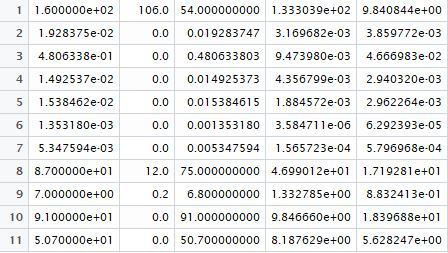
\includegraphics[width=0.75\textwidth]{chard.jpg}
  \label{}
  \end{figure}
And here is their histogram:
  \begin{figure}[H]
  \centering
  % Requires \usepackage{graphicx}
  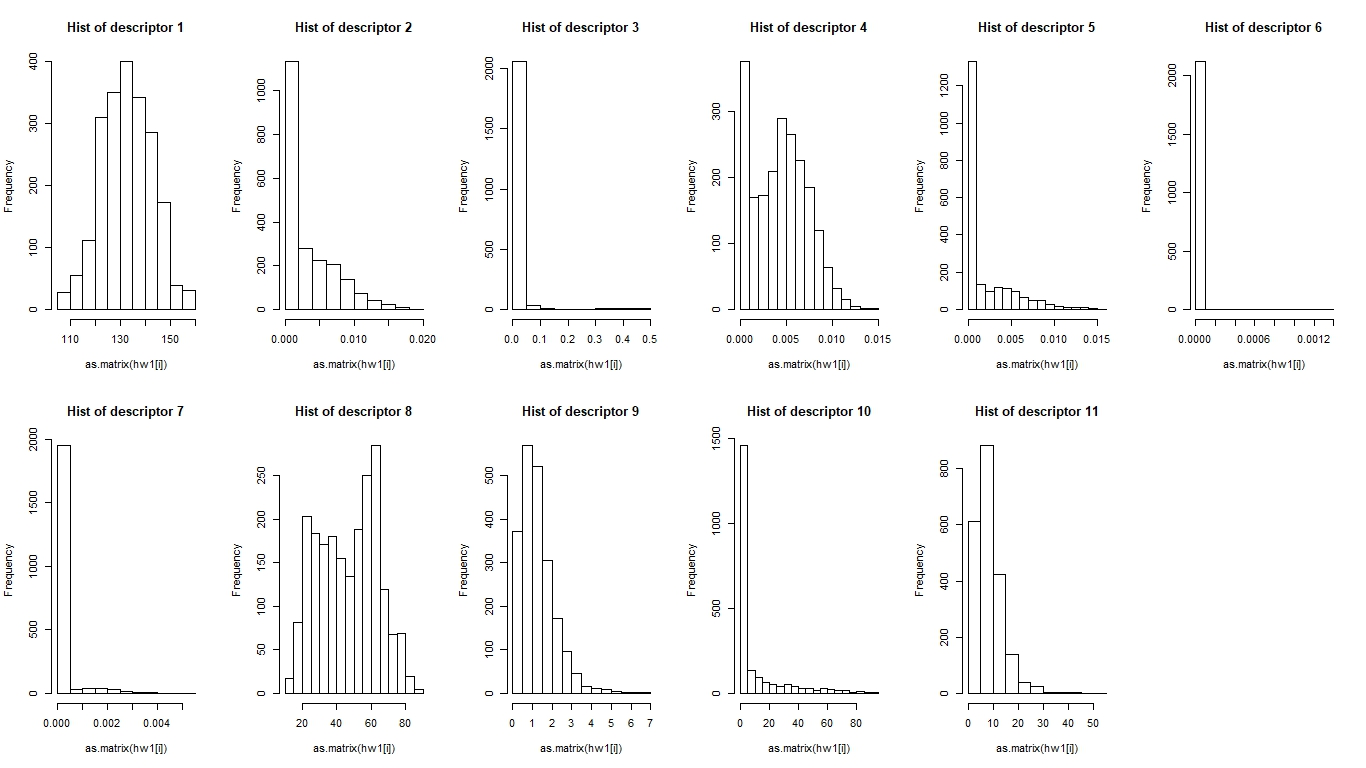
\includegraphics[width=1.2\textwidth]{Des.jpg}
  \caption{Histogram of descriptors}\label{}
  \end{figure}
\section{Problem 3}
Here are the histograms for each descriptor with 5 classes overlapped:
  \begin{figure}[H]
  \centering
  % Requires \usepackage{graphicx}
  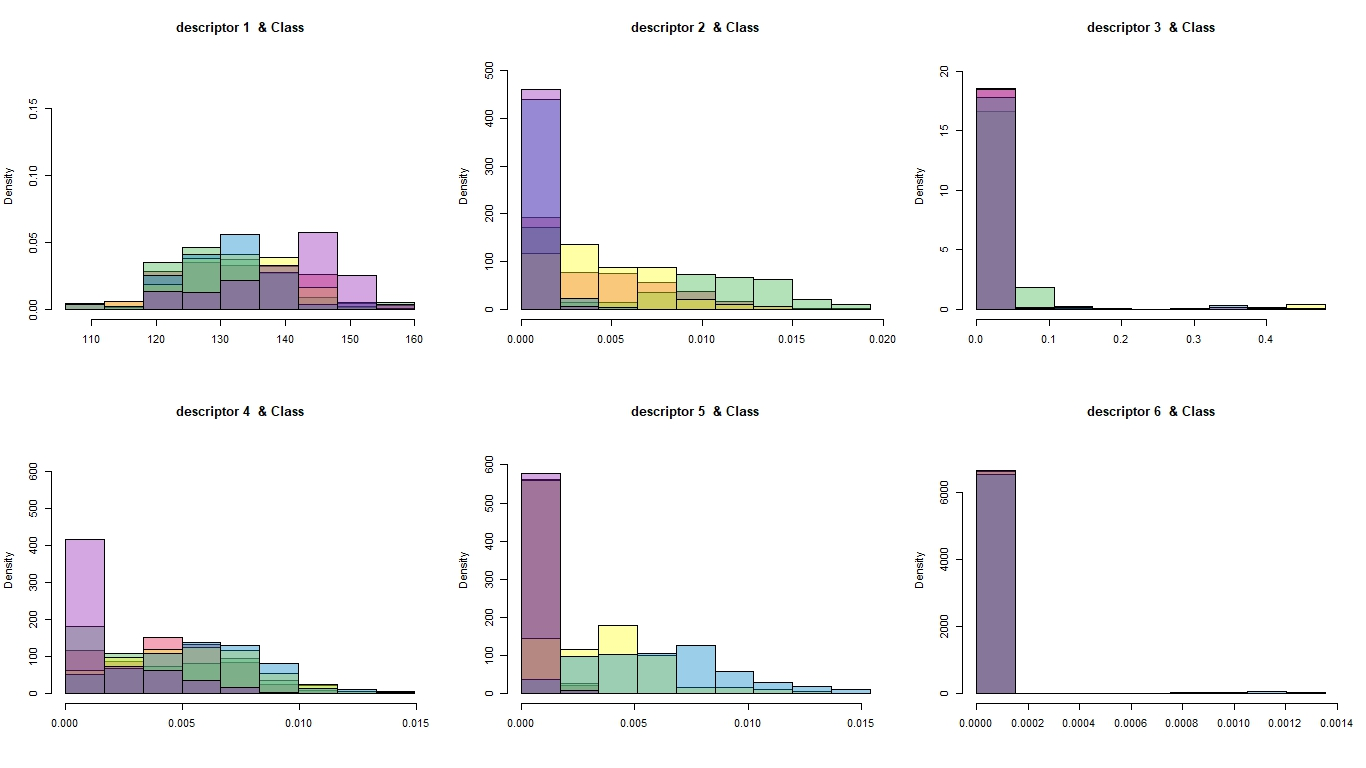
\includegraphics[width=1.35\textwidth]{DesCla1-6.jpg}
  \caption{Histogram of classes of descriptors 1-6}\label{}
  \end{figure}
  \begin{figure}[H]
  \centering
  % Requires \usepackage{graphicx}
  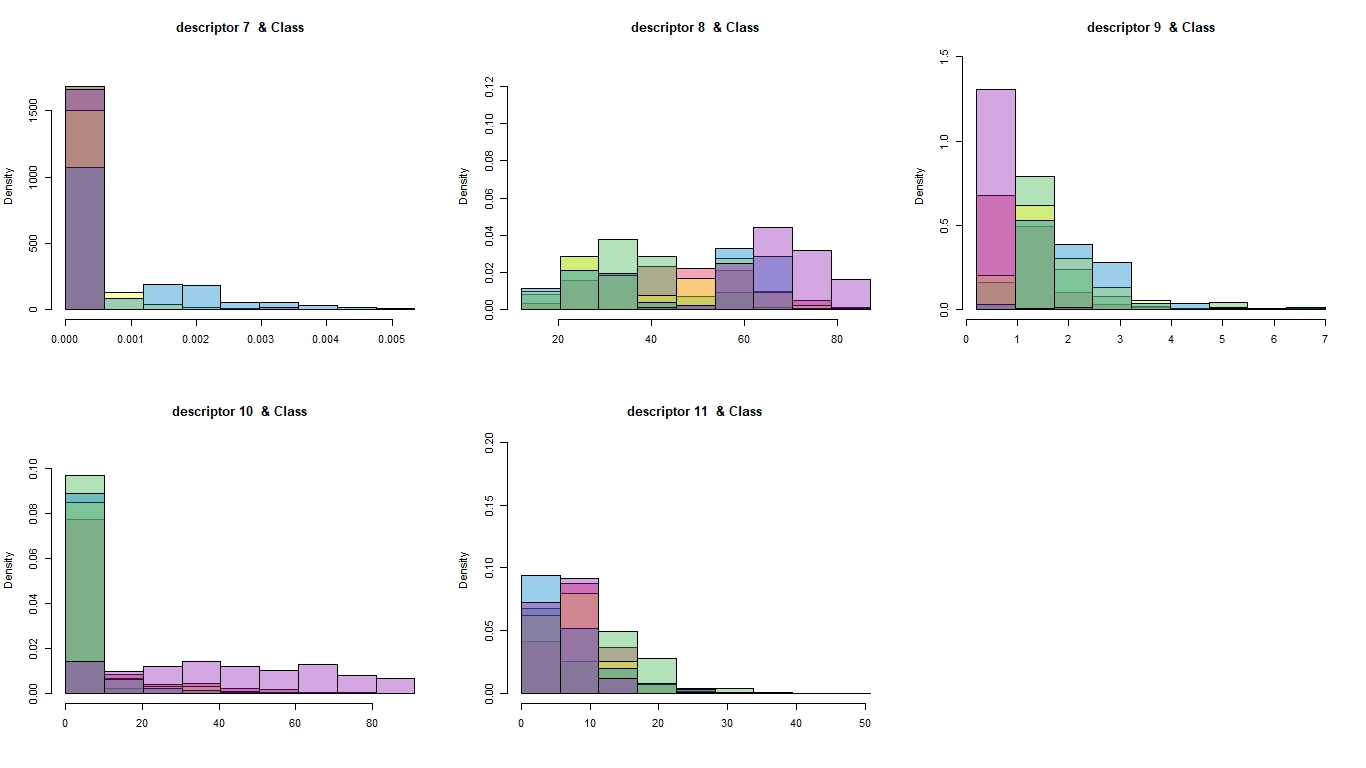
\includegraphics[width=1.35\textwidth]{DesCla7-11.jpg}
  \caption{Histogram of classes of descriptors 7-11}\label{}
  \end{figure}
According to the histograms, descriptor 2,3,5,8,9 and 10 are relatively more helpful to discriminate between some pairs of classes than the others.\\
The means and standard deviations are as follows:
  \begin{figure}[H]
  \centering
  % Requires \usepackage{graphicx}
  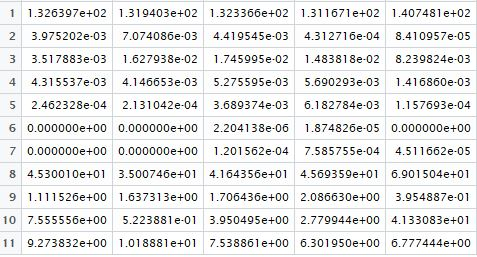
\includegraphics[width=0.75\textwidth]{mc.jpg}
  \caption{The means}\label{}
  \end{figure}
  \begin{figure}[H]
  \centering
  % Requires \usepackage{graphicx}
  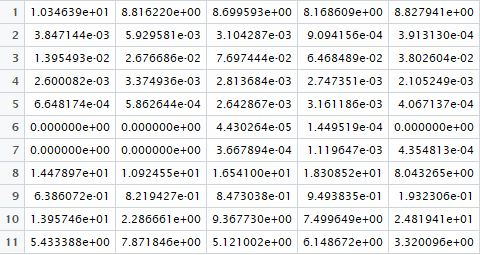
\includegraphics[width=0.75\textwidth]{sdc.jpg}
  \caption{The standard deviations}\label{}
  \end{figure}
With the t-test and the Kolmogorov-Smirnov test we can compare pairs of histograms and pairs of means. Because there are 11 descriptors, there are 220 tests in total.So here are only the p-values of these tests in descriptor1 given the $\alpha=0.05$, when $p<\alpha$, two histograms or two means are strongly distinct:
  \begin{figure}[H]
  \centering
  % Requires \usepackage{graphicx}
  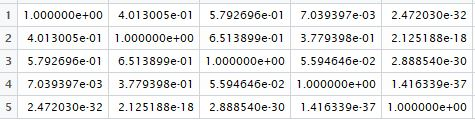
\includegraphics[width=0.75\textwidth]{t1.jpg}
  \caption{p-value of t-tests}\label{}
  \end{figure}
  \begin{figure}[H]
  \centering
  % Requires \usepackage{graphicx}
  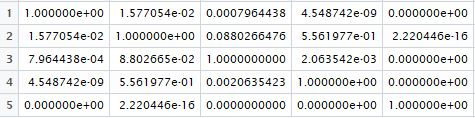
\includegraphics[width=0.75\textwidth]{ks1.jpg}
  \caption{p-value of K-S tests}\label{}
  \end{figure}
According to the results, some pairs are strongly distinct while some are not.\\
Relevant R codes are as follows:
\begin{lstlisting}[language=R]
class=list(class1,class2,class3,class4,class5)
t=array(0,c(5,5,11))
ks=array(0,c(5,5,11))
mc=array(0,c(11,5))
sdc=array(0,c(11,5))
for (i in 1:11){
  for (k in 1:5){
    mc[i,k]=mean(class[[k]][[i]])
    sdc[i,k]=sqrt(var(class[[k]][[i]]))
    for (m in 1:5){
      t[k,m,i]=t.test(as.matrix(class[[k]][[i]]),as.matrix(class[[m]][[i]]))$p.value
      ks[k,m,i]=ks.test(as.matrix(class[[k]][[i]]),as.matrix(class[[m]][[i]]))$p.value
      }
  }
}
\end{lstlisting}
\section{Problem 4}
The thing that principal component analysis(PCA) does is to transfer the original data to a basis that the features or characteristics of the data be relatively most reflected, and to decrease the redundancy of pairs of descriptors of the data. Follow this idea, we choose the directions that are linearly independent and the data's projections on which(the directions) are variance-maximized. Then this new basis is the eigenvector matrix of the original covariance matrix, and respective eigenvalues are the maximized variances. And if we think that to include relatively small eigenvalues and respective eigenvectors to the new basis is unnecessary, we could calculate the ratio:\[RAT_{j}=\frac{\sum\limits_{i=1}^{j}\lambda_{i}}{\sum\limits_{i=1}^{n}\lambda_{i}}\] where $j\leq n$ and $\lambda_{1},\cdots \lambda_{n}$ are all the eigenvalues rank descendingly.\\ We then choose the first j eigenvalues and eigenvectors as our new basis according to a given ratio level like 0.85,0.95,etc such that $RAT_{j}$ be grater than that given ratio level. This is my brief explanation of PCA.\\
The eigenvalues of this data set is 480.5307 171.3118 83.05912 27.88628 0.5497105 0.002137986 1.309506e-05 7.119464e-06 3.837938e-06 2.382227e-07 3.873138e-09. Display graphically as follow:
  \begin{figure}[H]
  \centering
  % Requires \usepackage{graphicx}
  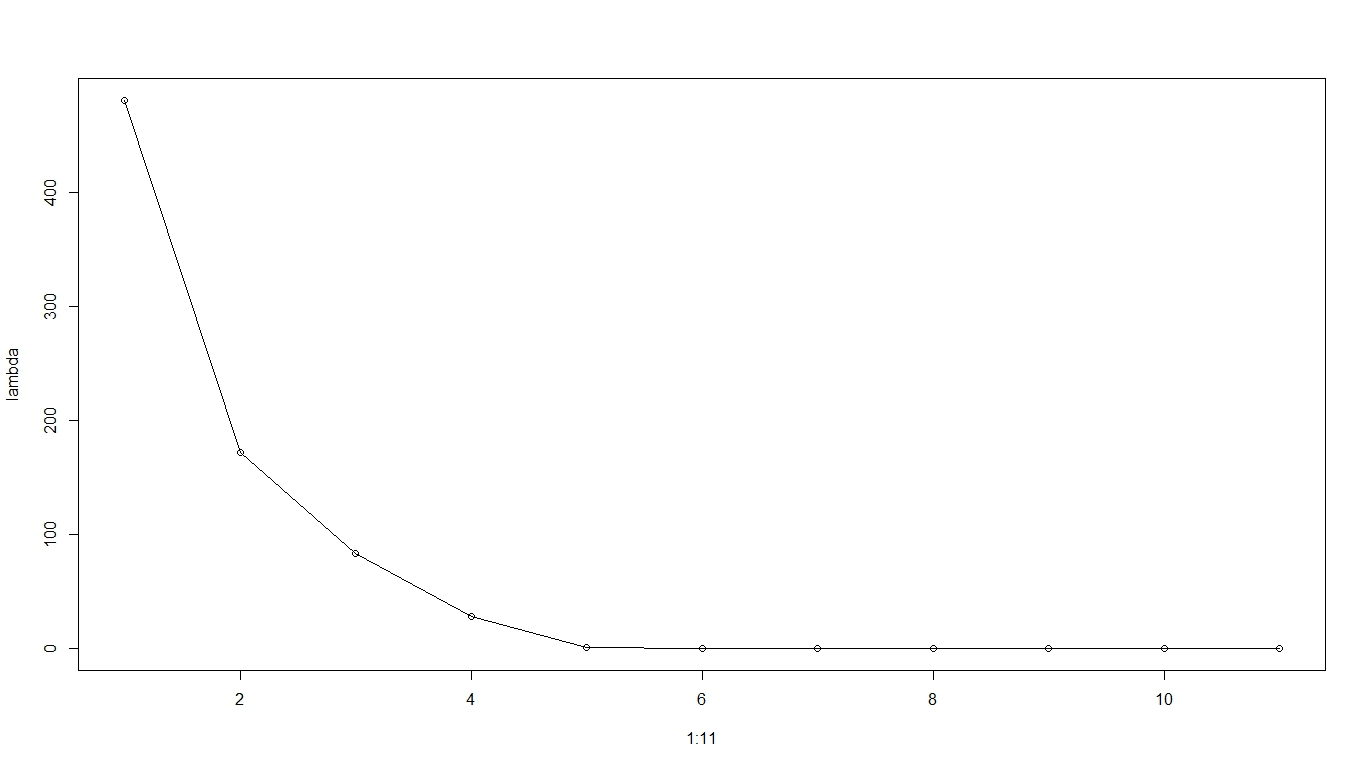
\includegraphics[width=1.0\textwidth]{lambda.jpg}
  \caption{eigenvalues}\label{}
  \end{figure}
The samllest j such that $RAT_{j}\geq0.95$ is 3, $RAT_{j}=0.9627451$. Display graphically as follow:
  \begin{figure}[H]
  \centering
  % Requires \usepackage{graphicx}
  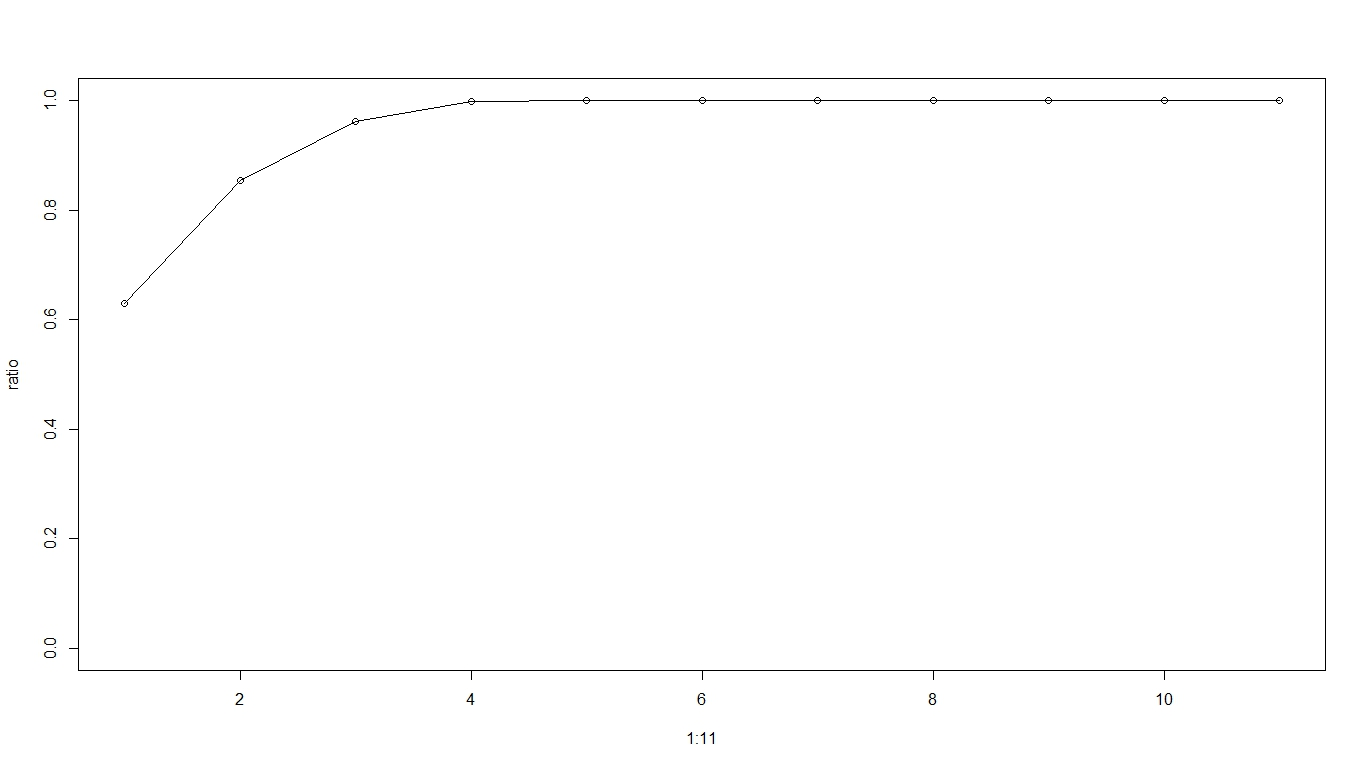
\includegraphics[width=1.0\textwidth]{ratio.jpg}
  \caption{ratio}\label{}
  \end{figure}
\section{Problem 5}
The scatter plot of basis \{W1,W2,W3\} is as follow:
  \begin{figure}[H]
  \centering
  % Requires \usepackage{graphicx}
  \includegraphics[width=1.0\textwidth]{scatter3d.jpg}
  \caption{ratio}\label{}
  \end{figure}
As we can see from the 3-dimensional scatter, points from different classes are separate mutually, and points from the same class are relatively concentrated. Although there are still some areas of mixed different color points, this is not a PCA could handle, but the classification by deep learning algorithms.
The scatter plots of basis \{W1,W2\} \{W1,W3\} \{W2,W3\} are as follows:
  \begin{figure}[H]
  \centering
  % Requires \usepackage{graphicx}
  \includegraphics[width=1.0\textwidth]{scatter12.jpg}
  \caption{ratio}\label{}
  \end{figure}
  \begin{figure}[H]
  \centering
  % Requires \usepackage{graphicx}
  \includegraphics[width=1.0\textwidth]{scatter13.jpg}
  \caption{ratio}\label{}
  \end{figure}
  \begin{figure}[H]
  \centering
  % Requires \usepackage{graphicx}
  \includegraphics[width=1.0\textwidth]{scatter23.jpg}
  \caption{ratio}\label{}
  \end{figure}
As we can see from the scatters, the basis \{W1,W2\} is the best 2d basis that reflects the classification(different colors of points are relatively most separate).
\end{document}
